\section{The Package Database ( \regdb)}
\label{sec:regdb}

The \regdb package is responsible for storing information about packages. In
this section we will cover in depth how this service works and how it is used.

This package provides storage, and querying facilities for package information.
This package does not provide any storage of actual packages. It is left to the
client of this package to perform this. This allows freedom in how contents is
stored, which may change between clients.

This package is consumed by both the \registry and the \cache packages. How
these packages communicate with the \regdb package will be covered in their
respective packages. The \regdb package essentially acts as a front-end to a
SQL database. We won't cover the technical details of how this works, but for
the remainder of this section we will cover what is stored and which facilities
this package provides.

The core data stored in the database is shown in Figure
\ref{fig:registry_database}. The core database model consists of three tables:
\txtl{package}, \txtl{package_dependency}, \txtl{package_versions}. The
\txtl{package} table describes a particular known package. Using any particular
entry in the \txtl{package} table, we may find all known versions of this
package. From a particular version of the package we may find all its known
dependencies.

\begin{figure}[H]
    \centering
    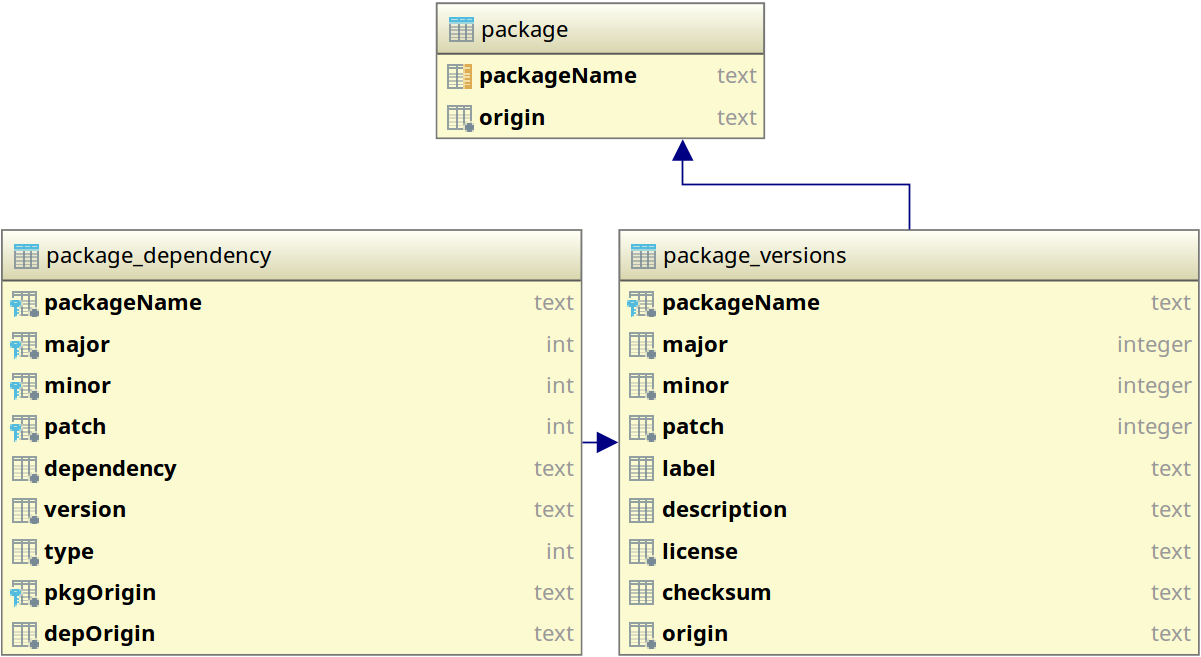
\includegraphics[width=1.0\textwidth]{pictures/regdb.png}
    \caption{The core database model used in the \regdb package}
    \label{fig:registry_database}
\end{figure}

The \txtl{origin} fields which appear in all three tables reference the origin
registry. This is used for handling both cross-registry dependencies, but also
for storing information about packages from different registries. The latter is
useful for cache-like services, which collect information from many different
registries.

Any particular package version also contains a \txtl{checksum} field. This
field can contain any generic checksum which can be serialized as text, that is
the actual checksum algorithm is defined by the client.

The remainder of the fields stored in the database simply mirror the most
important fields of the package manifests. Certain fields from the package
manifests, like the lifetime hooks, are left out of this database model. The
reason for this being lack of interest by clients. The remaining fields, like
name, description, license, are all of interest when it comes to
discoverability of packages.

Table \ref{tab:regdb_operations} shows the operations provided by the \regdb
package. Generally the operations provided by this package for querying
operations operate on a key matching either the \txtl{package} or
\txtl{package_versions} table. Operations that update the tables usually
operate on package manifests (typically provided by the \txtl{packages}
package).

\begin{table}[H]

\begin{longtable}[c]{@{}ll@{}}
\toprule
\begin{minipage}[b]{0.35\columnwidth}\raggedright\strut
Operation
\strut\end{minipage} &
\begin{minipage}[b]{0.59\columnwidth}\raggedright\strut
Description
\strut\end{minipage}\tabularnewline
\midrule
\endhead
\begin{minipage}[t]{0.35\columnwidth}\raggedright\strut
\txtl{query}
\strut\end{minipage} &
\begin{minipage}[t]{0.59\columnwidth}\raggedright\strut
Searches for packages matching a text query
\strut\end{minipage}\tabularnewline
\begin{minipage}[t]{0.35\columnwidth}\raggedright\strut
\txtl{checkIfPackageExists}
\strut\end{minipage} &
\begin{minipage}[t]{0.59\columnwidth}\raggedright\strut
Check if any package exists with name origin
\strut\end{minipage}\tabularnewline
\begin{minipage}[t]{0.35\columnwidth}\raggedright\strut
\txtl{getInfoAboutPackage}
\strut\end{minipage} &
\begin{minipage}[t]{0.59\columnwidth}\raggedright\strut
Lists all versions of a package matching name, origin, and possibly
version
\strut\end{minipage}\tabularnewline
\begin{minipage}[t]{0.35\columnwidth}\raggedright\strut
\txtl{compareWithNewest}
\strut\end{minipage} &
\begin{minipage}[t]{0.59\columnwidth}\raggedright\strut
Checks if a package manifest is newer than what is known by this
registry
\strut\end{minipage}\tabularnewline
\begin{minipage}[t]{0.35\columnwidth}\raggedright\strut
\txtl{insertNewPackage}
\strut\end{minipage} &
\begin{minipage}[t]{0.59\columnwidth}\raggedright\strut
Inserts a new version of a package manifest
\strut\end{minipage}\tabularnewline
\begin{minipage}[t]{0.35\columnwidth}\raggedright\strut
\txtl{createPackage}
\strut\end{minipage} &
\begin{minipage}[t]{0.59\columnwidth}\raggedright\strut
Creates a package with name and origin
\strut\end{minipage}\tabularnewline
\begin{minipage}[t]{0.35\columnwidth}\raggedright\strut
\txtl{getDependencies}
\strut\end{minipage} &
\begin{minipage}[t]{0.59\columnwidth}\raggedright\strut
Returns a list of dependencies for a package (name, origin, version)
\strut\end{minipage}\tabularnewline
\bottomrule
\end{longtable}

\caption{Operations provided by the \regdb package. Operations named changed
slightly for formatting reasons}

\label{tab:regdb_operations}

\end{table}
